\documentclass[t]{beamer}
\usetheme{NWERC2013}
\usepackage{graphicx}
\usepackage{eurosym}
\usepackage{listings}
\usepackage[T1]{fontenc}
\usepackage{lmodern}
\lstset{basicstyle=\ttfamily\scriptsize,columns=fullflexible}
\pgfdeclareimage[width=.30\paperwidth]{tudelft}{tudelft}
\pgfdeclareimage[width=.30\paperwidth]{tomtom}{tomtom}
\pgfdeclareimage[width=.85\paperwidth]{DW}{DW}
\title{}
\date{22nd of November 2013}
\begin{document}
\IntroFrame{The 2013 Northwestern Europe Regional Contest}{Welcome in Delft}
\section{Saturday}
\IntroFrame{The 2013 Northwestern Europe Regional Contest}{23rd of November 2013}
\subsection{Opening Ceremony}
\begin{frame}
	\frametitle{The goal of the contest}
	\begin{itemize}
	\item Solve as many problems in the least amount of time. 
	\item Balloons 
	\item Medals 
	\item World final places in Yekatarinaburg
 	\item IBM golden internship tickets 
\end{itemize}
\end{frame}
\begin{frame}
	\frametitle{Who is who}
	\begin{description}[l]
		\item[Red badges]{Contestants}
		\item[Yellow badges]{Coaches}
		\item[Blue badges, blue shirt]{Organisation}
		\item[Blue badges, orange shirt]{Runners}
		\item[Blue badges, pink shirt]{Technical Staff}
		\item[Blue-yellow badges]{Jury}
	\end{description}
\end{frame}
%\begin{frame}
%	\frametitle{Who is who}
%	\framesubtitle{The organisation and System}
%	\begin{itemize}
%		\item Bastiaan Gris\`el
%		\item Rebecca Jacobs
%		\item Lex Boleij
%		\item Martijn Rentmeester
%		\item Herman Banken
%		\item Mark Janssen
%		\item Freek van Tienen
%		\item Jeffrey de Lange
%	\end{itemize}
%\end{frame}
%\begin{frame}
%	\frametitle{Who is who}
%	\framesubtitle{The Jury}
%	\begin{itemize}
%	\item Xander Zonneveld
%	\item Peter Kluit
%	\item Marco Luken
%	\item Mathijs de Weerdt
%	\item Tommy F\"arnqvist
%	\item Boaz Pat-El
%	\item Boris de Wilde
%	\item Sidney Cadot
%	\item Joris van Rantwijk
%	\end{itemize}
%\end{frame}
\begin{frame}
	\frametitle{General Rules}
	\begin{itemize}
		\item No food or drinks in the contest hall
		\item No smoking in the building
		\item Always wear your badge
		\item Always wear your T-shirt in the contest area
		\item Watch out with balloons in the Conversation hall and Contest hall
	\end{itemize}
\end{frame}
% \SuccessFrame
\IntroFrame[tudelft]{Welcome to the\\Delft University of Technology}{Peter Kluit\\ Emiratus Professor of the Faculty EEMCS}
\IntroFrame{The 2013 Northwestern Europe Regional Contest}{Rebecca Jacobs}
\begin{frame}
	\frametitle{Schedule}
	\tableofcontents
\end{frame}
\begin{frame}[c]
	\frametitle{The contest site}
	\begin{pgfpicture}
		\pgftext[at=\pgfpoint{.1\paperwidth}{-.98\paperheight}, left, base]{\pgfuseimage{DW}}
	\end{pgfpicture}
\end{frame}
\begin{frame}
	\frametitle{Before the contest}
	\begin{itemize}
		\item Find your designated workspace
		\item Do not touch the computer hardware and problemset
		\item Don't bring bags, jackets, phones or other equipment to the contest area
		\item Don't bring your own paper, we will provide it
		\item Your PC will login when the contest starts
		\item Wear your T-shirt and badge on top
	\end{itemize}
	\begin{block}
		{Bring your TCR to the test session}
		Leave it at your workplace when the test session is over.\\
		Leave your DOMJUdge manual if you want it on paper during the contest.
	\end{block}
\end{frame}
\begin{frame}
	\frametitle{During the contest}
	\begin{itemize}
		\item Prints will be brought to you 
		\item If you have a question about the problem set, send a clarification request
		\item All other questions, ask your runner
	\end{itemize}
	\begin{block}
		{Yellow badges on the contest floor}
		\begin{itemize}
			\item During the contest \textbf{not} allowed
			\item During the test session allowed
		\end{itemize}
	\end{block}
\end{frame}
\begin{frame}
	\frametitle{After the test session}
	\begin{itemize}
	\item Leave your TCR at your workspace
	\item Take all your other papers, mascots and pens with you
	\item We will re-image your computers,\\ all settings will be reset to default 
	\item Lunch will be served in the conversation hall 
	\end{itemize}
\end{frame}
\begin{frame}
	\frametitle{Excursions}
	\begin{description}[l]
		\item[Beertasting] Meet in Conversation hall
		\item[Guided City Tour] Meet outside 
	\end{description}
\end{frame}
%\begin{frame}
%	\frametitle{Dinner}
%\end{frame}
\begin{frame}
	\frametitle{Sunday}
	\begin{itemize}
	\item Be on time for the Last Minute remarks at 09:00
	\item Wear you badge and T-Shirt
	\item Coaches are not allowed in the area around the Contest Hall 
	\item Lunch will be served at your workspace
	\end{itemize}
\end{frame}
\begin{frame}
	\frametitle{Coaches on Sunday}
	\begin{description}
		\item[11:00] General Coach Meeting
		\item[12:30] Nordic Coach Meeting
		\item[13:00] German Coach Meeting
		\item[13:30] Benelux Coach Meeting 
		\item[14:00] UK Coach Meeting
	\end{description}
	Problemsets will be available and coaches can compete in the online contest.
\end{frame}
%\QuestionsFrame
\subsection{System Introduction}
\IntroFrame{System Introduction}{Mark Janssen}
\begin{frame}
	\frametitle{Contents}
		\begin{itemize}
		\item General
		\item Quickstart
		\item Software
		\item Languages
		\item What to do in case of problems
		\item Q\&A
	\end{itemize}
\end{frame}
\begin{frame}[fragile]
\frametitle{General}
	\begin{itemize}
		\item Running DOMjudge 3.4.2-NWERC2013
		\item Separate (semi)live online contest (see \url{2013.nwerc.eu})
		\item Online scoreboard for actual contest
		\item IRC channel: \url{irc.ch.tudelft.nl}, \url{#nwerc}
	\end{itemize}
\end{frame}
\begin{frame}
	\frametitle{DOMjudge quickstart: team interface}
	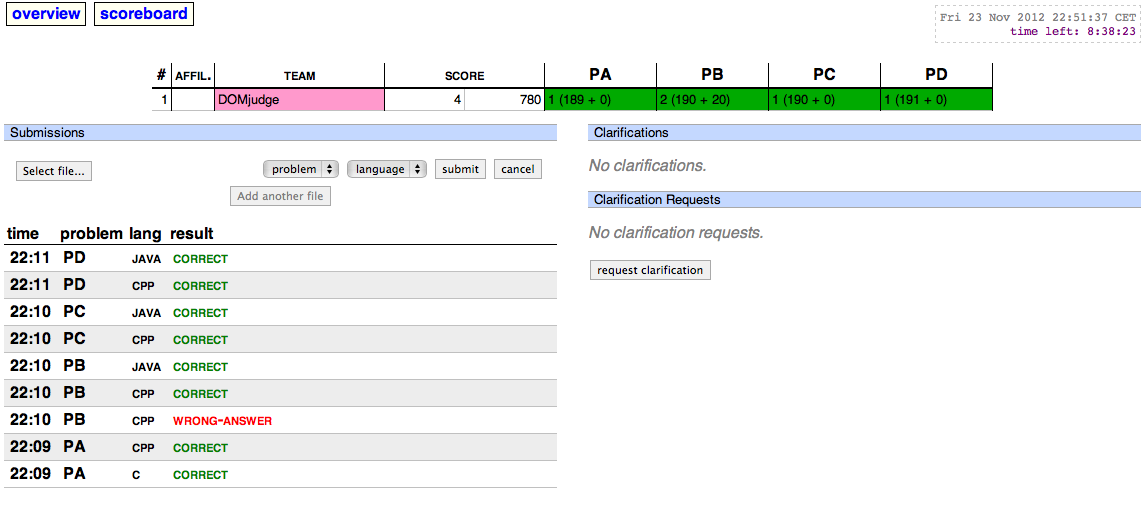
\includegraphics[width=90mm]{teaminterface.png}
	\end{frame}
\begin{frame}[fragile]
\frametitle{DOMjudge quickstart: submission}
	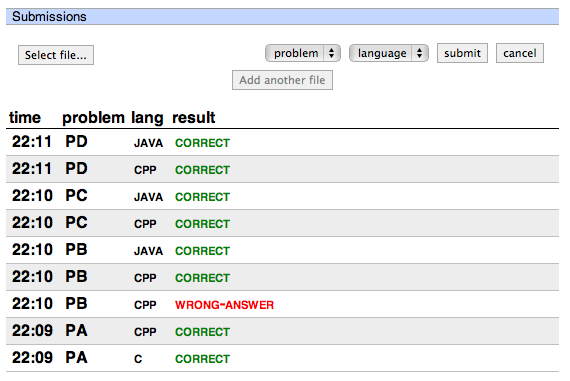
\includegraphics[width=90mm]{submissions.png}
	\\Or command line:
	\begin{lstlisting}
		submit --help
	\end{lstlisting}
\end{frame}
\begin{frame}
	\frametitle{DOMjudge quickstart: clarification requests}
	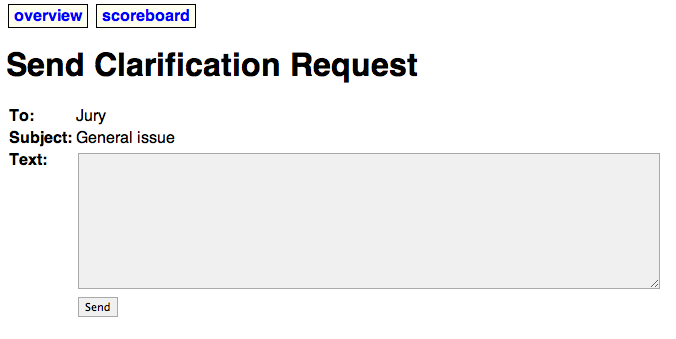
\includegraphics[width=90mm]{clarreq.png}
\end{frame}
\begin{frame}
	\frametitle{Software}
	\begin{itemize}
	\item Debian Linux 7 (Wheezy, amd64)
	\end{itemize}
	\begin{itemize}
		\item Xfce4 as default desktop
		\item Compilers and editors installed
		\item Sample input+output files available in home directory
		\item Web browser (Iceweasel) set up for DOMjudge
		\item Sublime Text 2 and IntelliJ installed (under /opt)
	\item Documentation (C, C++, Java) via browser bookmarks
		\begin{itemize}
			\item GNU C Library Documentation
			\item STL C++ Documentation
			\item Oracle Java SE 7 Documentation
			\item C++ Reference (cppreference.com)
		\end{itemize}
	\end{itemize}
\end{frame}
\begin{frame}[fragile]
	\frametitle{Languages}
	\begin{itemize}
		\item 1,5GB memory limit
		\item ~300MB reserved for JVM overhead
		\item C (GCC 4.7.2):\\    \lstinline|gcc -g -Wall -O2 -std=gnu99 -static -pipe -o $DEST "$@" -lm|
		\item C++:\\  \lstinline|g++ -g -Wall -O2 -std=gnu++98 -static -pipe -o $DEST "$@"|
		\item C++11:\\\lstinline|g++ -g -Wall -O2 -std=c++11 -static -pipe -o $DEST "$@"|
		\item Java 7:
		\begin{itemize}
			\item Compilation: \lstinline|javac -encoding UTF-8 -d . "$@"|
			\item Runtime: \lstinline|java -Xrs -Xss8m -Xmx1272864k \$MAINCLASS|
		\end{itemize}
		\item Aliases available on the system:\\
		\lstinline|mygcc|, \lstinline|myg++|, \lstinline|myg11|, \lstinline|myjavac| and \lstinline|myjava|.
	\end{itemize}
\end{frame}
\begin{frame}
	\frametitle{If something goes wrong\ldots}
	\begin{itemize}
		\item Submit a clarification request through DOMjudge
		\item If not possible: ask your nearest runner!
	\end{itemize}
\end{frame}
\IntroFrame{Jury}{Herman Banken}
\begin{frame}
    \frametitle{Jury: General}
    \begin{itemize}
        \item Runtime limits: up to 15 seconds per test run;\\
              We do multiple test runs for each submission;\\
              We do not provide the number of testcases.
        \item If it's on your system, you can use it (Python, Perl, etc.)
        \item No fooling around, it can lead to disqualification.
        \item No launching of threads/processes.
        \item Javadoc will be available.
    \end{itemize}
\end{frame}

\begin{frame}[fragile]
    \frametitle{Jury: I/O}
	\begin{itemize}
		\item Read from \lstinline|stdin|, write to \lstinline|stdout|.
		\item The test input \textbf{does not} start with the number of test cases.
		\item The test input is a concatenation of separate test cases.
		\item We have some leeway with whitespace matching, but no guarantees. \\
		  The easiest way to prevent problems is to follow the output specification precisely, and not print extra lines, spaces, etc.
		\item All output lines should end with a newline.
		\item There is no \lstinline|PRESENTATION ERROR|.
		\item Required accuracy for floating point numbers is specified in the problem.
		      We check floating point numbers by value, not by string compare.
	 \end{itemize}
\end{frame}
\QuestionsFrame
\subsection{Test Session}
%\ProgramFrame{Test Session}
\begin{frame}
	\frametitle{Test Session}
	\begin{itemize}
		\item Find your designated workspace
		\item Do not touch the computer hardware and problemset
		\item Do not bring bags, jackets, phones or other equipment to the contest area
		\item Your PC will log in when the contest starts
		\item Leave your TCR at your workspace after the testsession
		\item Take all your other papers, mascots and pens with you
	\end{itemize}
\end{frame}
\subsection{Lunch}
\ProgramFrame{Lunch}
\subsection{Excursions}
\begin{frame}
	\frametitle{Excursions}
	\begin{description}[l]
		\item[Beertasting] Meet in Conversation hall
		\item[Guided City Tour] Meet outside 
	\end{description}
\end{frame}
\subsection{Talk by TomTom}
\IntroFrame[tomtom]{''TomTom -- Quicker Journeys through Algorithm Engeneering'' }{Dr. Heiko Schilling}
\subsection{Q\&A Test Session}
\IntroFrame{Q\&A Test Session}{}

\begin{frame}
	\frametitle{Contents}
		\begin{itemize}
		\item Jury
		\item System
		\item Organization
	\end{itemize}
\end{frame}


\begin{frame}
    \frametitle{Jury: Staplers}
	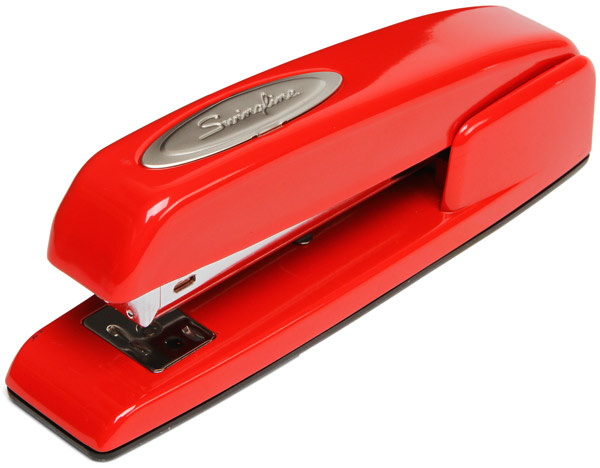
\includegraphics[width=100mm]{stapler.jpg}
\end{frame}

\begin{frame}[fragile]
    \frametitle{System}
    \begin{itemize}
        \item Installed: \lstinline|joe vim-gtk openjdk-7-source apcalc bc galculator time|
        \item \lstinline|myg11| alias works (as well as \lstinline|myg++11|).
        \item Java source is available; Eclipse documentation works.
        \item Sublime Text 2 is in \lstinline|/opt|.
        \item \lstinline|submit --help| is now more clear.
        \item Printing should work for all teams\\(through your editor or \lstinline|a2ps|).
        \item No extra GDB macros are added.
     \end{itemize}
\end{frame}

\begin{frame}
    \frametitle{Organisation}
    \begin{itemize}
        \item Pen and paper is at your workspace.
        \item Air conditioning should work.
        \item Do not touch the computer hardware before contest starts,\\
        	you will be logged on automatically.
        \item Bags, jackets, phones and other equipment should left with coaches.
        \item Limited space available for storing valuables.
        \item Be here at 9:00 tomorrow morning!
     \end{itemize}
\end{frame}

\QuestionsFrame
\subsection{Dinner}
\ProgramFrame{Dinner}
\section{Sunday}
\subsection{Last Minute Remarks}
\subsection{Contest}
\subsection{Drinks}
\subsection{Award Ceremony}
\QuestionsFrame
\end{document}
